% Auth: Nicklas Vraa
% Docs: https://github.com/NicklasVraa/LiX

\documentclass{textbook}
\usepackage{graphicx}
\usepackage{subcaption}
\usepackage{float}

\hypersetup{
    colorlinks=true,
    linkcolor=blue,
    filecolor=magenta,      
    urlcolor=blue,
    pdftitle={Overleaf Example},
    pdfpagemode=FullScreen,
    }
    
\lang      {english}
\title     {Kentech Tutorial of Advancing Sustainability through Computational Chemistry Methods}
% \subtitle  {Kentech CCP 2023 Summer - Let's Roll a Dice: Monte Carlo Simulation 101}
\author     {KENTECH EF Chemistry}
\date       {\today}
% \cover*    {resources/textbook_front.png}{resources/textbook_back.pdf}
% \license   {CC}{by-nc-sa}{3.0}{The Company}
% \isbn      {978-0201529838}
% \publisher {JK}
% \edition   {Summer}{2023}
% \dedicate  {Kentech Community}{JK}
% \thank     {JK}
% \keywords  {computational chemistry, Monte Carlo}
% \note{JK}
% \maketitle
\begin{document}

\h*{Kentech Tutorial of Advancing Sustainability through Computational Chemistry Methods} %Non-Numbered Heading
In today's advancing landscape of science and engineering,  computational methods have become an essential tool. With the advent of artificial intelligence and machine learning, their importance is only further heightened, where they are increasingly being used to make groundbreaking discoveries and advances.

This tutorial is a collaborative effort that showcases the work of undergraduate students of Kentech, with a focus on the computational elements of Chemistry and Energy Engineering. This document will be updated on a regular basis, reflecting the ongoing learning and innovative activities taking place at Kentech.

Yet, this tutorial is more than just a collection of academic activities. It is envisaged as a platform facilitating the exchange of knowledge and experiences amongst students. Through such discourse, I aspire to foster a positive and dynamic learning culture at Kentech. As we navigate this path of scientific exploration, we are committed to learning, sharing, and collectively evolving.

In the spirit of collaboration, all developed codes will be shared openly via GitHub, further enriching the learning experience and ensuring an open-source approach to our scientific journey.

August 6, 2023

Jeongmin Kim (and ChatGPT-4)

\toc
\h{Monte Carlo Simulation 101}
This chapter was developed through a CCP program in 2023 summer entitled "Let's Roll a Dice: Monte Carlo Simulation 101" with the support of Kentech Residential College Education Center.

Our motto was "Practice fuels progress".

All the codes are freely available at \url{our GitHub page}{https://github.com/Jeongmin0658/kentech_tutorial}. \textcolor{magenta}{JK: this page is still private.}

\textcolor{red}{\textbf{To-Do List}:
    \begin{itemize}
        \item Front and Back cover pages - photos that summarize our activities
        \item Contributors: Insert your photo, self-introduction, and experience in CCP this summer at your fav position.
        \item Prepare code examples to share with this tutorial on GitHub: incomplete codes to practice and answer.
    \end{itemize}
}

\hh{Editorial}
Page for our Editor, Seohyun Kim.

\hh{Contributors}
\begin{figure}[H]
  \centering
    \begin{minipage}{0.9\textwidth} % Set the width of the entire figure here
  \begin{subfigure}{0.25\textwidth}
    \includegraphics[width=\textwidth]{example-image-a}
    \caption{Contributor A1}
  \end{subfigure}
  \hfill
  \begin{subfigure}{0.25\textwidth}
    \includegraphics[width=\textwidth]{example-image-b}
    \caption{Contributor A2}
  \end{subfigure}
  \hfill
  \begin{subfigure}{0.25\textwidth}
    \includegraphics[width=\textwidth]{example-image-c}
    \caption{Contributor A3}
  \end{subfigure}
  
  % You can add some vertical space in between the rows
  \vspace{0.5cm}

  % The next row
  \begin{subfigure}{0.25\textwidth}
    \includegraphics[width=\textwidth]{example-image-a}
    \caption{Contributor B1}
  \end{subfigure}
  \hfill
  \begin{subfigure}{0.25\textwidth}
    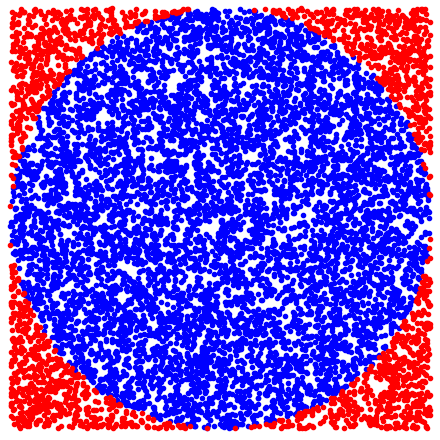
\includegraphics[width=\textwidth]{resources/textbook_front.png}
    \caption{Hi all. I'm Pi. My academic interest for now is apricot recipes. It was my pleasure to be computed this summer. Enjoy this tutorial!}
  \end{subfigure}
  \hfill
  \begin{subfigure}{0.25\textwidth}
    \includegraphics[width=\textwidth]{example-image-c}
    \caption{Contributor B3}
  \end{subfigure}

    % You can add some vertical space in between the rows
  \vspace{0.5cm}

  % The next row
  \begin{subfigure}{0.25\textwidth}
    \includegraphics[width=\textwidth]{example-image-a}
    \caption{Contributor C1}
  \end{subfigure}
  \hfill
  \begin{subfigure}{0.25\textwidth}
    \includegraphics[width=\textwidth]{example-image-b}
    \caption{Contributor C2}
  \end{subfigure}
  \hfill
  \begin{subfigure}{0.25\textwidth}
    \includegraphics[width=\textwidth]{example-image-c}
    \caption{Contributor C3}
  \end{subfigure}

    % You can add some vertical space in between the rows
  \vspace{0.5cm}

  % The next row
  \begin{subfigure}{0.25\textwidth}
    \includegraphics[width=\textwidth]{example-image-a}
    \caption{Contributor C1}
  \end{subfigure}
  \hfill
  \begin{subfigure}{0.25\textwidth}
    \includegraphics[width=\textwidth]{example-image-b}
    \caption{Contributor C2}
  \end{subfigure}
  \hfill
  \begin{subfigure}{0.25\textwidth}
    \includegraphics[width=\textwidth]{example-image-c}
    \caption{Contributor C3}
  \end{subfigure}

  \caption{Contributors of 2023 summer edition}
  \end{minipage}
\end{figure}

\newpage

\hh{Basics 1: GitHub and Google CoLab}
This part is about how to use GitHub and CoLab. Should be very practical
Byungchan, June, Suhyun
\textcolor{magenta}{JK: Again, should be very practical. Anyone can use both tools if they follow what's illustrated in this section.}

\hh{Basics 2: Latex and Overleaf}
This part is about how to use overleaf and Latex. Should be very practical as well. Maybe include the Usages below.
\textcolor{magenta}{JK: This might not be part of this summer edition.}


\hh{Scientific coding with Python}
This part contains the activity of the first meeting.
Minyong, Eunseo, Seojin 
\textcolor{magenta}{JK: before discussing the examples, better to introduce simple Python statements for the very beginners, such as for-statement, if-statement, etc. Pick code examples to share on GitHub that answer the questions.}

\hh{Pi estimation}
This part contains the activity of the second meeting.
Seohyun, Gahyun
\textcolor{magenta}{JK: Introduce an idea where how we compute Pi numerically, and one method is Monte Carlo.}

\hh{Ising model}
This part contains the activity of the third meeting.
Hansu, Jisu


\h{Usages}

\hh{Subheading}

\hhh{Subsubheading}

\hh{Formats}
Formats that you may use: \b{bold}, \i{italic}, \s{strikethrough}, \u{underlined}, and code: \c{def func(a,b): return a+b}

\hh{Mathematics}
Below is an example of how to write an equation~\ref{2dmf} in this tutorial.
    \math{2dmf}{
    \langle M \rangle = \tanh\bigg(\frac{NJ}{k_BT}\langle M\rangle\bigg)
    }

\hh{Code Blocks}
Here is an example to put a code~\ref{evol} in this tutorial.

    %\code{label}{language}{
    % your code...
    %}{caption}
    \code{evol}{python}{
    def plot_evolution(system, snapshot_interval):
        """
        Plot the evolution of the Ising model, showing both the state of the lattice and the total magnetization
        """
        fig = plt.figure(figsize=(2*len(system.snapshots), 5))  # adjust the figure size here
        grid = plt.GridSpec(2, len(system.snapshots), hspace=0.2, wspace=0.2)
    
        # Plot lattice snapshots
        for i, snapshot in enumerate(system.snapshots):
            ax = fig.add_subplot(grid[0, i])
            ax.imshow(snapshot, cmap='gray')
            ax.set_title(f"Step {i * snapshot_interval}")
            if i != 0:
                ax.get_yaxis().set_visible(False)  # Removes the y-axis for snapshots that are not the leftmost
    
        # Plot magnetization
        ax2 = fig.add_subplot(grid[1, :])
        ax2.plot(system.magnetization)
        ax2.set_ylim(-1.1, 1.1)
        #ax2.set_title('Total Sum of Spins vs. MC Step')
        ax2.set_xlabel('MC Step * total number of spins')
        ax2.set_ylabel('Normalized total magnetization')
        ax2.grid(True)
    
        # Draw markers and arrows on magnetization plot
        snapshot_steps = [i*snapshot_interval for i in range(len(system.snapshots))]
        ax2.plot(snapshot_steps, [system.magnetization[i] for i in snapshot_steps], 'ro')  # Plot markers
    
        plt.show()
    }
    {This is a code to plot how the normalized total magnetization as a function of Monte Carlo step.}

\hh{Tables}
Below is an example of table.

    \tabs{my_table}{cols}{
    This & is & a & cool & table \\
    1    & 2  & 3 & 4    & 5     \\
    a    & b  & c & d    & e     \\
    }
    {Table description.}

\hh{Figures}
Nullam massa nunc, sollicitudin id eleifend vitae, pellentesque sit amet lectus. Morbi vestibulum leo quis tempor lacinia. Praesent vitae est ante. Fusce dignissim in urna et posuere.

    \fig{my_svg}{0.3}{resources/textbook_front.png}
    {This is a figure for pi estimation.}

Integer sed metus malesuada, volutpat urna condimentum, aliquet metus. Phasellus interdum.

\hh{Lists}
Elit vel sagittis luctus, arcu libero pellentesque nisi, sed consectetur quam neque a elit. Donec consectetur cursus nulla eu feugiat. Lorem ipsum dolor sit amet, consectetur adipiscing elit.

    \items{
    ¤ Something.
    ¤ Another thing.
        \items{
        ¤ A subitem.
        ¤ Another subitem.
            \items*{
            ¤ A subitem.
            ¤ Another subitem.
            }
        }
    ¤ And another item.
    ¤ Last item.
    }

Pellentesque et blandit leo. Sed lacinia, sapien sit amet posuere tempor, eros nunc consectetur massa, id pulvinar diam nulla ut felis. Nam id iaculis dui. Pellentesque dapibus, ligula non gravida euismod, risus odio feugiat quam, id ultrices tellus est et dui.

\hh{Referencing}
Here is a hyperlink to a \url{webpage}{https://www.overleaf.com/}. This is a reference to \r{2dmf}, and this refers to \r{my_svg}. You can also refer to headings like \r{Tables}. \R{evol} is a capitalized variant. For all references, both the name and number are links.

\end{document}
